
%(BEGIN_QUESTION)
% Copyright 2010, Tony R. Kuphaldt, released under the Creative Commons Attribution License (v 1.0)
% This means you may do almost anything with this work of mine, so long as you give me proper credit

Suppose this DC electric motor refuses to start as it should when the pushbutton switch is pressed.  A voltmeter subsequently connected between test points {\bf E} and {\bf D} in this circuit always registers 0 volts, whether the switch is pressed or not:

$$\includegraphics[width=15.5cm]{i04620x01.eps}$$

Identify the likelihood of each specified fault for this circuit.  Consider each fault one at a time (i.e. no coincidental faults), determining whether or not each fault could independently account for {\it all} measurements and symptoms in this circuit.

% No blank lines allowed between lines of an \halign structure!
% I use comments (%) instead, so that TeX doesn't choke.

$$\vbox{\offinterlineskip
\halign{\strut
\vrule \quad\hfil # \ \hfil & 
\vrule \quad\hfil # \ \hfil & 
\vrule \quad\hfil # \ \hfil \vrule \cr
\noalign{\hrule}
%
% First row
{\bf Fault} & {\bf Possible} & {\bf Impossible} \cr
%
\noalign{\hrule}
%
% Another row
Pushbutton switch failed open &  &  \cr
%
\noalign{\hrule}
%
% Another row
Motor winding(s) failed open &  &  \cr
%
\noalign{\hrule}
%
% Another row
Relay coil failed shorted &  &  \cr
%
\noalign{\hrule}
%
% Another row
Pushbutton switch failed shorted &  &  \cr
%
\noalign{\hrule}
%
% Another row
15 amp fuse blown &  &  \cr
%
\noalign{\hrule}
%
% Another row
0.5 amp fuse blown &  &  \cr
%
\noalign{\hrule}
%
% Another row
Voltage source dead &  &  \cr
%
\noalign{\hrule}
} % End of \halign 
}$$ % End of \vbox

\vfil 

\underbar{file i04620}
\eject
%(END_QUESTION)





%(BEGIN_ANSWER)

% No blank lines allowed between lines of an \halign structure!
% I use comments (%) instead, so that TeX doesn't choke.

$$\vbox{\offinterlineskip
\halign{\strut
\vrule \quad\hfil # \ \hfil & 
\vrule \quad\hfil # \ \hfil & 
\vrule \quad\hfil # \ \hfil \vrule \cr
\noalign{\hrule}
%
% First row
{\bf Fault} & {\bf Possible} & {\bf Impossible} \cr
%
\noalign{\hrule}
%
% Another row
Pushbutton switch failed open &  & $\surd$ \cr
%
\noalign{\hrule}
%
% Another row
Motor winding(s) failed open &  & $\surd$ \cr
%
\noalign{\hrule}
%
% Another row
Relay coil failed shorted &  & $\surd$ \cr
%
\noalign{\hrule}
%
% Another row
Pushbutton switch failed shorted &  & $\surd$ \cr
%
\noalign{\hrule}
%
% Another row
15 amp fuse blown & $\surd$ &  \cr
%
\noalign{\hrule}
%
% Another row
0.5 amp fuse blown &  & $\surd$ \cr
%
\noalign{\hrule}
%
% Another row
Voltage source dead & $\surd$ &  \cr
%
\noalign{\hrule}
} % End of \halign 
}$$ % End of \vbox

%(END_ANSWER)





%(BEGIN_NOTES)

{\bf This question is intended for exams only and not worksheets!}.

%(END_NOTES)

